\newpage
\section{Question 5}
	\subsection{}
		\subsubsection{Workspace}
			\begin{figure}[position = here]
			\begin{centering}
				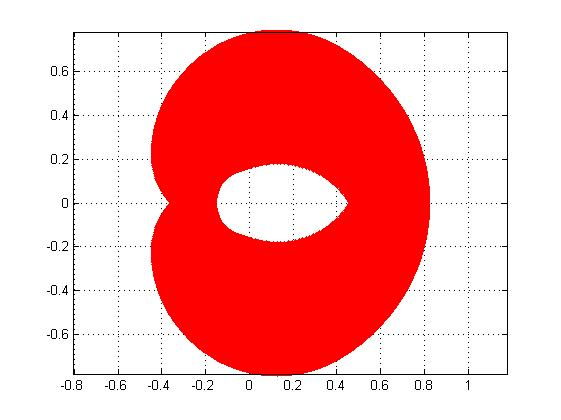
\includegraphics[scale=0.5]{q5_workspace2}\\
				\caption [WSpace]{Workspace Plot (See Appendix A [9.4.i])}
			\end{centering}
			\end{figure}
		
		\subsubsection{Configuration Space}
			\begin{figure}[position = here]
			\begin{centering}
				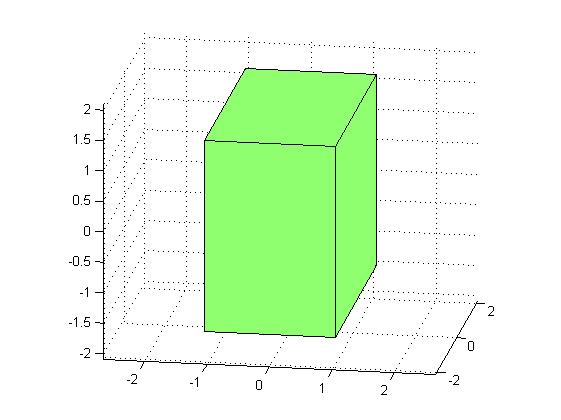
\includegraphics[scale=0.5]{q5_config_space}\\
				\caption [CSpace]{Configuration Space Plot (See Appendix A [9.4.ii])}
			\end{centering}
			\end{figure}
	\pagebreak		
	\subsection{Singularities}
%		we believe the values for ....
Considering link L1 and link L2, take end point of link L2 as P(x,y)

$x = L_{1} \cos\theta_{1} + L_{2}\cos(\theta_{1}+\theta_{2}))$\\
$x' = (-L_{1}\sin\theta_{1}- L_{2}\sin(\theta_{1}+\theta_{2}))\theta' - L_{2}\sin(\theta_{1}+\theta_{2})\theta_{2}'$\\
$y = L_{1}\sin\theta_{1} + L_{2}\sin(\theta_{1} + \theta_{2})$\\
$y' = (L_{1}\cos\theta_{1}- L_{2}\cos(\theta_{1}+\theta_{2}))\theta' - L_{2}\cos(\theta_{1}+\theta_{2})\theta_{2}'$\\
\vspace{5mm}

$$
 \begin{pmatrix}
 x'\\y'
 \end{pmatrix} =
\begin{pmatrix}
- L_{1}\sin\theta_{1} - L_{2}\sin(\theta_{1} + \theta_{2}) & -L_{2}\sin(\theta_{1} + \theta_{2})\\
L_{1}\cos\theta_{1} + L_{2}\cos(\theta_{1} + \theta_{2}) & L_{2}\cos(\theta_{1} + \theta_{2})
\end{pmatrix}\cdot
\begin{pmatrix}
\theta_{1}'\\\theta_{2}'
\end{pmatrix}
$$

$$
\begin{pmatrix}
x'\\y'
\end{pmatrix} =
\begin{pmatrix}
J_{1}
\end{pmatrix}\cdot
\begin{pmatrix}
\theta_{1}'\\\theta_{2}'
\end{pmatrix}
$$

\hspace{40mm} where $J_{1}$ = 
$$
\begin{pmatrix}
- L_{1}\sin\theta_{1} - L_{2}\sin(\theta_{1} + \theta_{2}) & -L_{2}\sin(\theta_{1} + \theta_{2})\\
L_{1}\cos\theta_{1} + L_{2}\cos(\theta_{1} + \theta_{2}) & L_{2}\cos(\theta_{1} + \theta_{2})
\end{pmatrix}
$$\\

$det(J_{1}) = (- L_{1}\sin\theta_{1} - L_{2}\sin(\theta_{1} + \theta_{2}))\cdot(L_{2}\cos(\theta_{1} + \theta_{2})) + (L_{2}\sin(\theta_{1} + \theta_{2}))\cdot(L_{1}\cos\theta_{1} + L_{2}\cos(\theta_{1} + \theta_{2}))$\\

$det(J_{1}) = L_{1}L_{2}\sin\theta_{3}$\\
\newline
\vspace{5mm}

Similarly we can find that
\newline
\vspace{5mm}
$\therefore det(J_{1}) = L_{2}L_{3}\sin\theta_{3}$\\
\vspace{2mm}

Finding singularities
Singularities occurs when $det⁡(J)=0$\\

For $J_{1}$:\\

$det(J_{1}) = L_{2}L_{3}\sin\theta_{3} = 0$

$\therefore $ when $ \theta_{3} = 0$ or $\pi$

However, the range of $\theta{3}$ must be between $(-\pi/2)$ and $(\pi/2)$\\
$\therefore \theta_{3} = 0$\\
\newline
\vspace{5mm}
Similarly for $J_{2}$:\\

$det(J_{2}) = L_{1}L_{2}\sin\theta_{2} = 0$

$\therefore $ when $ \theta_{2} = 0$ or $\pi$

However, the range of $\theta{2}$ must be between $(-2\pi/3)$ and $(2\pi/3)$\\
$\therefore \theta_{2} = 0$

So for the whole system singularities occurs according to the intersection of results of A & B:\\
$\theta_{2} = 0$ and $ \theta_{2} = 0$